\documentclass[a4paper,11.5pt]{article}
\usepackage[textwidth=170mm, textheight=230mm, inner=20mm, top=20mm, bottom=30mm]{geometry}
\usepackage[normalem]{ulem}
\usepackage[utf8]{inputenc}
\usepackage[T1]{fontenc}
\PassOptionsToPackage{defaults=hu-min}{magyar.ldf}
\usepackage[magyar]{babel}
\usepackage{amsmath, amsthm,amssymb,paralist,array, ellipsis, graphicx,float}
%\usepackage{marvosym}

\makeatletter
\renewcommand*{\mathellipsis}{%
	\mathinner{%
		\kern\ellipsisbeforegap%
		{\ldotp}\kern\ellipsisgap%
		{\ldotp}\kern\ellipsisgap%
		{\ldotp}\kern\ellipsisaftergap%
	}%
}
\renewcommand*{\dotsb@}{%
	\mathinner{%
		\kern\ellipsisbeforegap%
		{\cdotp}\kern\ellipsisgap%
		{\cdotp}\kern\ellipsisgap%
		{\cdotp}\kern\ellipsisaftergap%
	}%
}
\renewcommand*{\@cdots}{%
	\mathinner{%
		\kern\ellipsisbeforegap%
		{\cdotp}\kern\ellipsisgap%
		{\cdotp}\kern\ellipsisgap%
		{\cdotp}\kern\ellipsisaftergap%
	}%
}
\renewcommand*{\ellipsis@default}{%
	\ellipsis@before
	\kern\ellipsisbeforegap
	.\kern\ellipsisgap
	.\kern\ellipsisgap
	.\kern\ellipsisgap
	\ellipsis@after\relax}
\renewcommand*{\ellipsis@centered}{%
	\ellipsis@before
	\kern\ellipsisbeforegap
	.\kern\ellipsisgap
	.\kern\ellipsisgap
	.\kern\ellipsisaftergap
	\ellipsis@after\relax}
\AtBeginDocument{%
	\DeclareRobustCommand*{\dots}{%
		\ifmmode\@xp\mdots@\else\@xp\textellipsis\fi}}
\def\ellipsisgap{.1em}
\def\ellipsisbeforegap{.05em}
\def\ellipsisaftergap{.05em}
\makeatother

\usepackage{hyperref}
\hypersetup{
	colorlinks = true	
}

\DeclareMathOperator{\Int}{int}
\DeclareMathOperator{\tg}{tg}
\DeclareMathOperator{\ctg}{ctg}
\DeclareMathOperator{\Th}{th}
\DeclareMathOperator{\sh}{sh}
\DeclareMathOperator{\ch}{ch}
\DeclareMathOperator{\sgn}{sgn}
\DeclareMathOperator{\arc}{arc}
\DeclareMathOperator{\arctg}{arc tg}
\DeclareMathOperator{\arcctg}{arc ctg}

\begin{document}
	%%%%%%%%%%%RÖVIDÍTÉSEK%%%%%%%%%%
	\setlength\parindent{0pt}
	\def\s{\hspace{0.2mm}\vphantom{\beta}}
	\def\Z{\mathbb{Z}}
	\def\Q{\mathbb{Q}}
	\def\R{\mathbb{R}}
	\def\C{\mathbb{C}}
	\def\N{\mathbb{N}}
	\def\Ra{\overline{\mathbb{R}}}
	
	\def\sume{\displaystyle\sum_{n=1}^{+\infty}}
	\def\sumn{\displaystyle\sum_{n=0}^{+\infty}}
	
	\def\narrow{\underset{n\rightarrow+\infty}{\longrightarrow}}
	\def\limn{\displaystyle\lim_{n\to +\infty}}
	\def\limx{\displaystyle\lim_{x\to +\infty}}
	
	
	\theoremstyle{definition}
	\newtheorem{theorem}{Tétel}[subsection] 
	
	\theoremstyle{definition}
	\newtheorem{definition}[theorem]{Definíció} 
	\newtheorem{example}[theorem]{Példa} 
	\newtheorem{task}[theorem]{Feladat} 
	\newtheorem{note}[theorem]{Megjegyzés}
	\newtheorem{revision}[theorem]{Emlékeztető}
	%%%%%%%%%%%%%%%%%%%%%%%%%%%%%%%%%%%%%%%%%%%%%%%%%%%%%%%%%%%%%%%%%%%%%
	\begin{center}
		{\LARGE\textbf{Analízis II.}}
		
		{\Large Előadás jegyzet}
		
		11. óra.
	\end{center}
	A jegyzetet \textsc{Umann} Kristóf készítette Dr. \textsc{Szili} László  előadásán. (\today)
	
	%Külön köszönet jár \textsc{Csonka} Szilviának a képek elkészítésért.
	%\bigskip
	
	Tantárgyi honlap: \url{http://numanal.inf.elte.hu/~szili/Oktatas/An2_BSc_2016/index_An2_2016.htm}
	\section{Információk}
	\begin{itemize}
		\item Kint vannak a honlapon a zh témakörei.
		\item kis zh-ból \textbf{nincs}, azaz {\LARGE\textbf{NINCS}} javítás vagy pótlás. Méltányolható esetben nyilván lehet ezalól kivétel, ez ügyben az ember a gyakvezzel beszéljen először.
		\item Megajánlott vizsgajegyhez kell gyakorlati jegy, azonban ez megszerezhető gyakuv-n is, így ha az elméleti része a ZH-nak sikeres volt, de a gyakorlati része nem, akkor még mindig lehetséges a megajánlott vizsgajegy megszerzése.
		\item a bizonyításokra a zh-n \textbf{4 pont}ot lehet legfeljebb szerezni. Ha
		\begin{itemize}
			\item A tétel kimondása rossz, a bizonyítás 0 pont.
			\item A bizonyítás pontosságától, minőségétől függően lehet 1 és 4 pont között szerezni pontokat, ha a kimondás helyett.
		\end{itemize}
		A megajánlott vizsgajegyhez legalább \textbf{5 pont} kell.
		\item hogyha az első zh-n a tételbizonyítás 4 pontos volt, elég a tételkimondás is a másodikon.
	\end{itemize}
	\section{Határozott integrál (hat. int.)}
	Motiváció: Síkidom területe. Középiskolában megadtunk egy egységnégyzetet, ennek  területét megadtuk együtt, és minden más síkidomot ennek függvényében felírni. Ebből kiindulva megpróbáltuk a téglalap, parallelogramma terület meghatározni, parallelogramma megfelezésével meg tudtuk kapni a háromszög területét, és háromszögekből sok érdekes síkidomot tudtuk alkotni. 
	
	Azonban a kör területének meghatározásakor csak megjegyezttük, hogy az $r^2\cdot\pi$, de azt nem, hogy miért.
	
	\smallskip
	Hogyan tudjuk az analízis módszereivel meghatározni egy síkidom területét?
	\smallskip
	
	\textbf{Problémáink:
	}\begin{itemize}
		\item terület fogalma
		\item terület kiszámítása
	\end{itemize}
	Ez fog elvezetni minket a határozott integrálhoz.
	
	\smallskip
	\textbf{Természetes ötlet:} próbáljuk meg ezt a síkidomot közelíteni valamilyen ismert síkidommal! Mondjuk azt, hogy $f:[a,b]\to\R$, és $f\geq 0$. 
	
	\begin{figure}[!h]
		\centering
		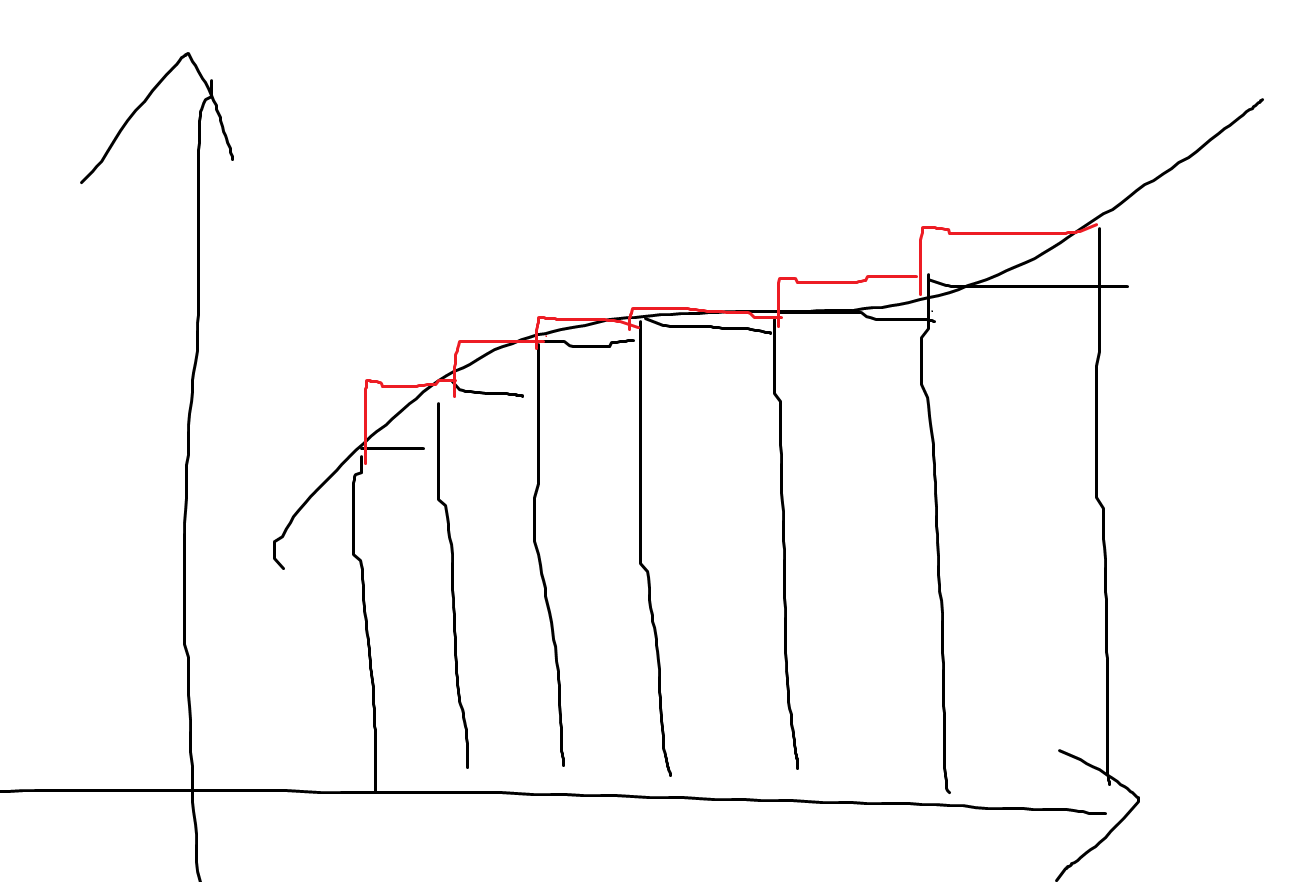
\includegraphics[height=3cm]{kepek/teglalap.png}
		\caption{Paintben csináltam, dont hate.}\label{}
	\end{figure}
	
	Az ábrán látható, hogy valamilyen felosztásokkal igyekszünk közelíteni a függvényhez: a fekete téglalapokkal alulról, a pirosakkal felülről (un. beírt és körülírt téglalapokkal). Mennél sűrűbbre vesszük a felosztást, annál közelebb érünk a függvényhez!
	\subsection{A határozott integrál elemzése}
	Egyenlőre ilen függvényekre:
	\begin{definition}
		$a,b\in\R,\quad a<b$.
		\[ K[a,b]:=\{f:[a,b]\to\R\ |\ f \text{\quad korlátos.} \} \]
	\end{definition}
	\begin{definition}
		$a,b\in\R,\quad a<b;\quad n\in\N.$ Az $[a,b]$ intervallum egy felosztása:
		\[ \tau:=\{ x_0,x_1,\ldots,x_n \}\subset[a,b],\quad \text{ha}\quad a=x_0<x_1<\dots<x_n=b \]
		Jel: $\mathcal{F}[a,b]:$ az $[a,b]$ felosztásainak halmaza.
	\end{definition}
	\begin{definition}
		$\tau_1, \tau_2\in\mathcal{F}[a,b]$ és $\tau_1\subset\tau_2$, akkor a $\tau_2$ a $\tau_1$ egy \textbf{finomítása}.
	\end{definition}
	\begin{definition}
		$f\in K[a,b], \quad \tau\in\mathcal{F}[a,b].$
		
		%(beírt téglalapok összege)
		\[ s(f;\tau):=\sum\left(\inf_{x\in[x_i,x_{i+1}]} f(x)\right)(x_{i+1}-x_i) \]
		Ezt nevezzük az $f$ függvény $\tau$-hoz tartozó alsó közelítő összegnek.
		\[ S(f;\tau):=\sum\left(\sup_{x\in[x_i,x_{i+1}]} f(x)\right)(x_{i+1}-x_i) \]
		Ezt nevezzük az $f$ függvény $\tau$-hoz tartozó felső közelítő összegnek.
	\end{definition}
	\begin{note}
		$s(f,\tau)$ a beírt, $S(f;\tau)$ a körülírt téglalapok területének összege.
	\end{note}
	Figyeljük meg, hogy geometriai fogalmakra egyáltalán nem volt szükségünk! Mi fog történni ezekkel, ha finomítjuk a felosztást?
	\begin{theorem}
		$f\in K[a,b],\quad \tau_1,\tau_2\in\mathcal{F}[a,b].$
		\begin{enumerate}
			\item Ha $\tau_1\subset\tau_2$ ($\tau_2$ felosztás finomabb $\tau_1$-nél)\quad $\Rightarrow\quad \left\{
			\begin{gathered}
				s(f;\tau_1)\leq s(f;\tau_2)\\
				S(f;\tau_1)\geq S(f;\tau_2)\\
			\end{gathered}\right.$
			\item $\forall \tau_1,\tau_2\quad \Rightarrow\quad s(f;\tau_1)\leq S(f;\tau_2)$.
		\end{enumerate}
		\begin{note}
			Hogyan tudnánk bebizonyítani? ha véges sok pont van, sima teljes indukció elég lenne.
		\end{note}
		\begin{note}
			1-hez: ábrás cucc, nem volt időm megrajzolni.
			
			2-höz: $\tau:=\tau_1\cup \tau_2$ és alkalmazható 1-et.
		\end{note}
		\textit{Bizonyítás:}
		\begin{enumerate}
			\item \[ \{ s(f;\tau)\ | \ \tau\in\mathcal{F}[a,b] \}\quad \text{felülről korlátos.} \]
			\[ \exists\sup\{ s(f;\tau)\ | \ \tau\in\mathcal{F}[a,b]=:I_*(f)<+\infty \} \]
			Az $f$ függvény Darboux-féle alsó integrálja.
			\item \[ \{ S(f;\tau)\ | \ \tau\in\mathcal{F}[a,b] \}\quad \text{alulról korlátos.} \]
			\[ \exists\inf\{ S(f;\tau)\ | \ \tau\in\mathcal{F}[a,b]=:I^*(f)<+\infty \} \] 
			Az $f$ függvény Darboux-féle felső integrálja.
		\end{enumerate}
	\end{theorem}
	\begin{theorem} (triviális megállapítás)
		\[ \forall f\in K[a,b],\quad \exists I_*(f), I^*(f)\quad \text{és}\quad I_*(f)\leq I^*(f). \]
	\end{theorem}
	\begin{definition}
		$a,b\in\R,\quad a<b.$ Az $f:[a,b]\to\R$ korlátos függvényt \textbf{Riemann-intergálható} $[a,b]$-n ($f\in R[a,b]$), ha 
		\[ I_*(f)=I^*(f). \]
		Ezt a számot az $f$ függvény $[a,b]$-n vett Riemann-integráljának nevezzük, és így jelöljük:
		\[ \int_a^bf\quad \text{vagy}\quad \int_a^bf(x)\, dx. \]
	\end{definition}
	Ez sok kérdést vet fel:
	\begin{itemize}
		\item Milyen függvények integrálhatóak?
		\item Hogyan lehet egyáltalán ezt kiszámolni?
		\item Mi a fenére lehet alkalmazni?
	\end{itemize}
	\begin{example}
		Nem integrálható az alábbi függvény:
		\[ f(x):=
		\begin{cases}
			1,\quad x\in\Q\\
			0,\quad x\in \Q^*
		\end{cases} \]
		$f\notin R[0,1],\quad$ ui. $I_*(f)=0,\quad  I^*(f)=1.$
	\end{example}
	\begin{definition}
		$a,b\in\R,\quad a<b,\quad f:[a,b]\R,\quad f\geq 0.$ 
		Az
		\[ A:=\{ (x,y)\ | \ a\leq x\leq b,\quad 0\leq y\leq f(x) \} \]
		síkidomnak van területe, ha $f\in R[a,b]$. Ekkor:
		\[ t(A):=\int_a^bf \]
		valós számot a síkidom \textbf{terület}ének nevezzük.
	\end{definition}
	\begin{note}
		$f:[a,b]\to\R,\quad f\geq 0$
		\begin{figure}[H]
			\centering
			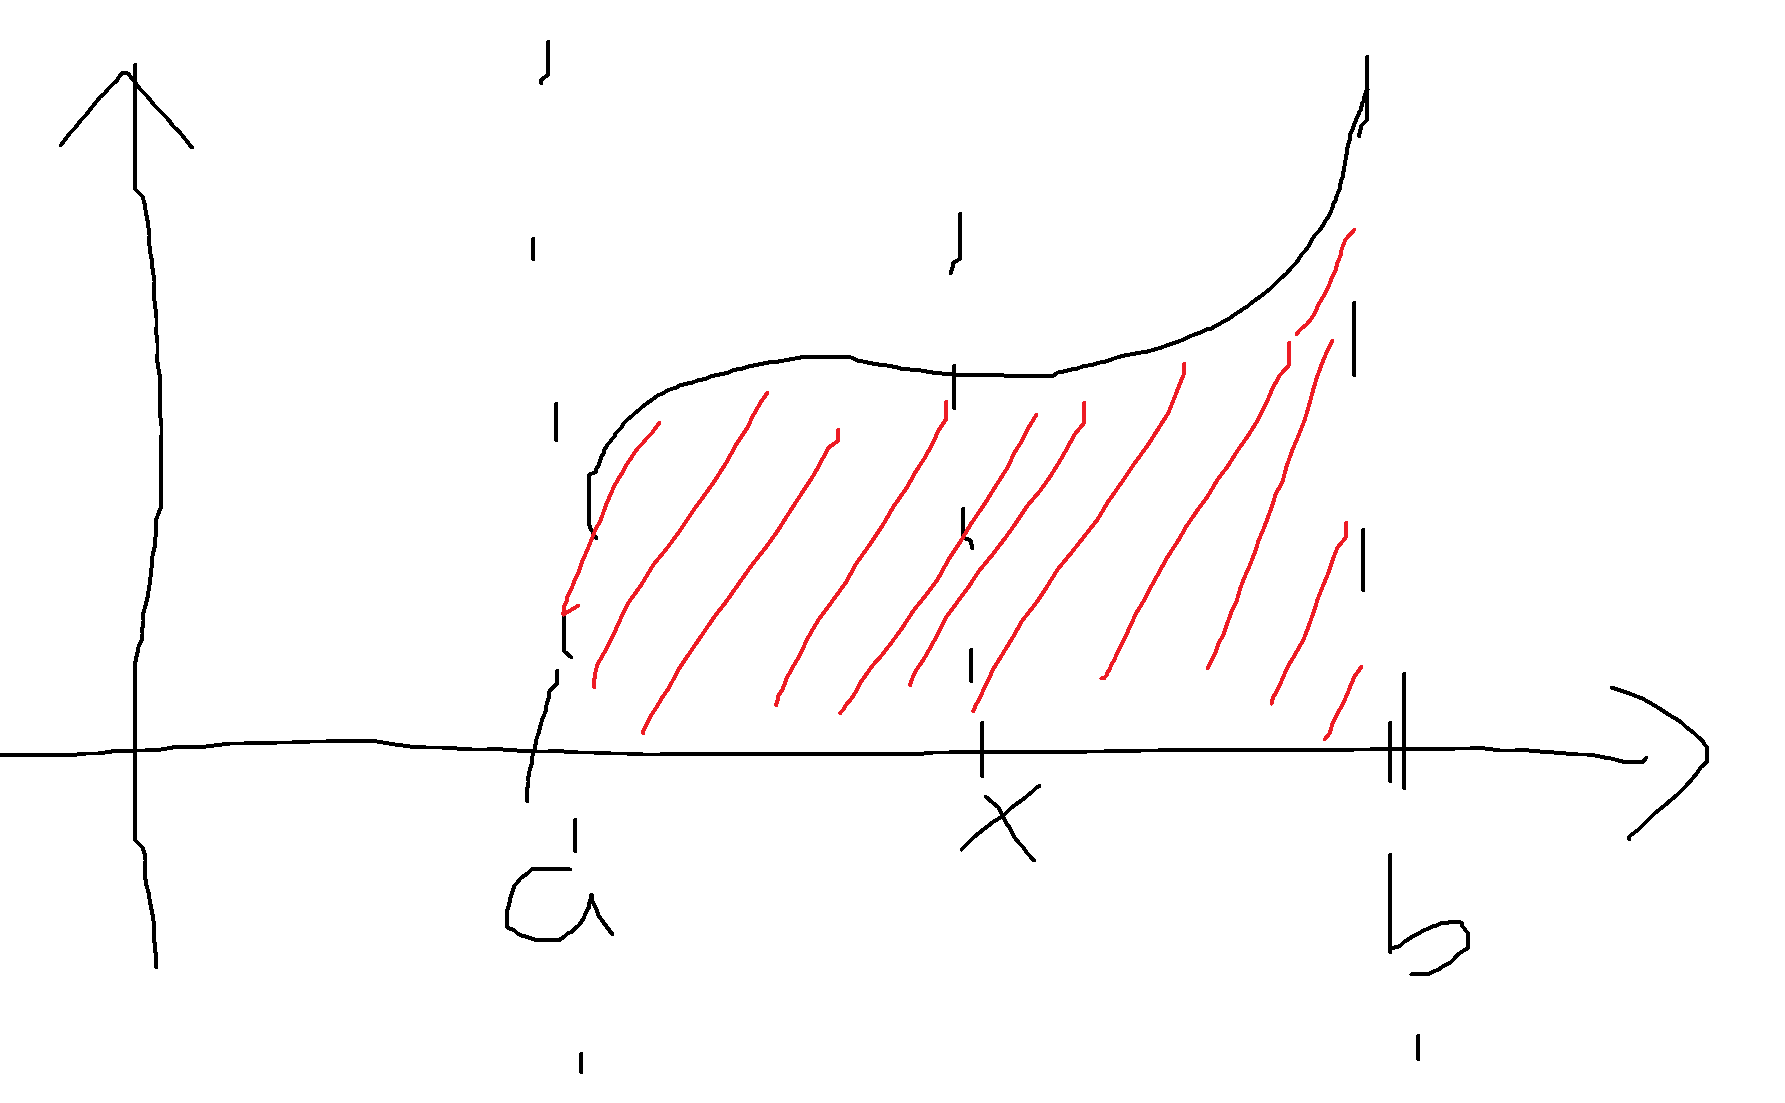
\includegraphics[height=5cm]{kepek/terulet.png}
			\caption{Paintben csináltam, dont hate.}\label{}
		\end{figure}
	\end{note}
	\subsection{Ekvivalens átfogalmazások}
	\begin{definition}
		$f\in K[a,b],\quad \tau\in\mathcal{F}[a,b]$.
		\[ \varOmega(f;\tau):=\quad S(f;\tau)-s(f;\tau) \]
		az $f$ függvény $\tau$-hoz tartozó \textbf{oszcillációs összeg}e.
	\end{definition}
	\begin{note}
		\begin{figure}[H]
			\centering
			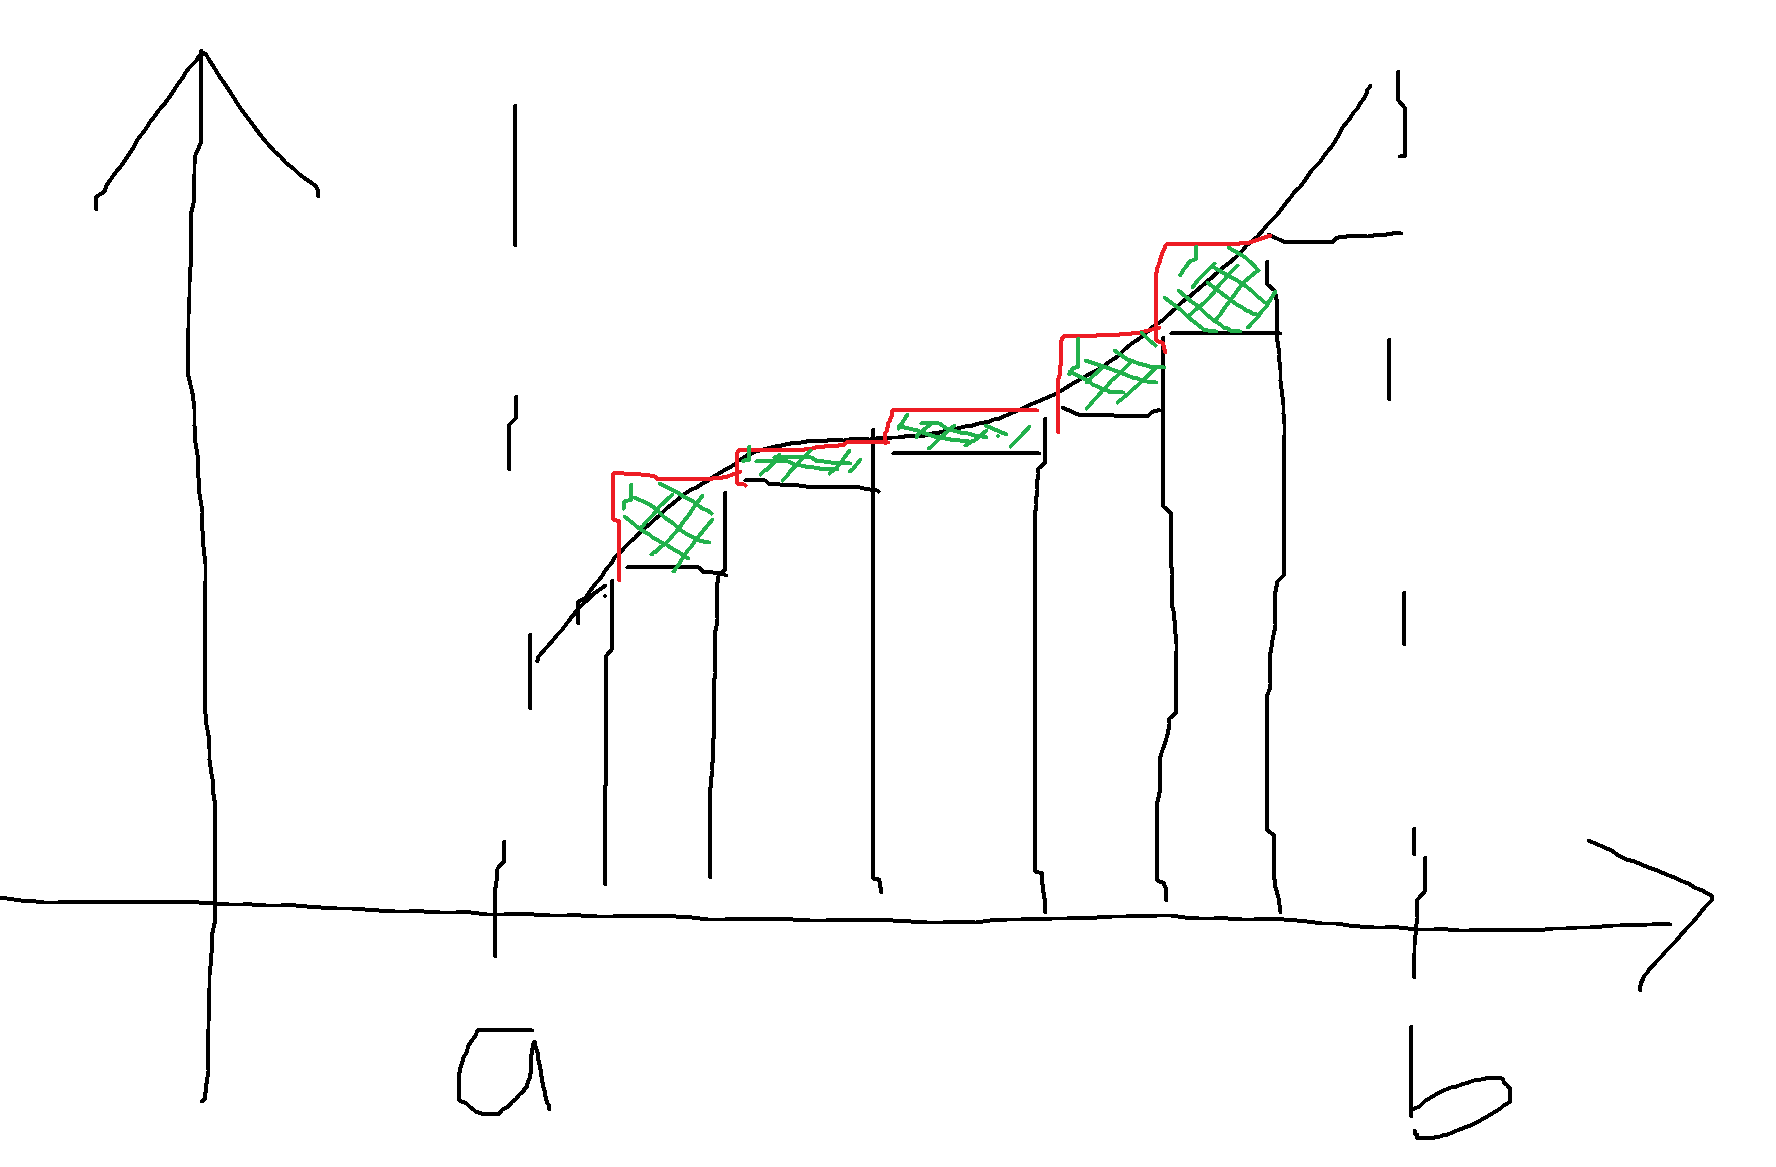
\includegraphics[height=5cm]{kepek/tau.png}
			\caption{Paintben csináltam, dont hate. Akkor mondjuk, hogy valaminek van területe, ha a zöld rész tetszőlegesen kicsi lehet.}\label{}
		\end{figure}
	\end{note}
	\begin{theorem}
		\[ f\in R[a,b]\quad \Leftrightarrow\quad \begin{gathered}
			\forall\varepsilon>0\quad \exists\tau\in\mathcal{F}[a,b],\\
			\varOmega(f;\tau)<\varepsilon\\
			\text{(az oszcillációs összeg tetszőlegesen kicsi lehet)}
		\end{gathered} \]
		\textit{Bizonyítás:}
		
		\fbox{$\Rightarrow:$}
		\[ I_*(f)=I^*(f)=:I \]
		$\varepsilon>0$ tetszőleges, szuprémum definíciójából:
		\[ \varepsilon>0\text{-hoz}\quad \exists\tau_1\in\mathcal{F}[a,b],\quad I-\frac{\varepsilon}{2}<s(f;\tau_1)\leq I \]
		\[ \varepsilon>0\text{-hoz}\quad \exists\tau_2\in\mathcal{F}[a,b],\quad I<S(f;\tau_1)\leq I+\frac{\varepsilon}{2} \]
		Legyen \fbox{$\tau:=\tau_1\cup\tau_2$}.
		\[ I-\frac{\varepsilon}{2}<s(f;\tau_1)\leq s(f;\tau)\leq S(f;\tau)\leq S(f;\tau_2)<I+\frac{\varepsilon}{2} \]
		\[ \Rightarrow\quad\varOmega(f;\tau)= S(f;\tau)-s(f;\tau)<\varepsilon. \]
		\fbox{$\Leftarrow:$}
		\[ \varepsilon>0\text{-hoz}\quad \exists\tau\in\mathcal{F}[a,b]\quad \varOmega(f;\tau)<\varepsilon \]
		\[ \varOmega(f;\tau)=S(f;\tau)-s(f;\tau)\geq I^*(f)-I_*(f)\geq 0 \]
		\[ \Rightarrow\quad 0\leq I^*(f)-I_*(f)<\varepsilon \]
		\[ \Rightarrow\quad I^*(f)-I_*(f)=0\quad \Rightarrow\quad I^*(f)=I_*(f)\Rightarrow\quad f\in R[a,b].\quad \blacksquare \]
	\end{theorem}
	\begin{definition}
		$f\in K[a,b];\quad  \tau:=\{ a=x_0<x_1<\ldots<x_n=b \}\in \mathcal{F}[a,b]$.
		\[ \xi=(\xi_0,\xi_1,\xi_{n-1}):\quad \xi_k\in[x_k,x_{k+1}]\quad (k=0,1,\ldots,n-1) \]
		\[\sigma(f;\tau,\xi):= \sum_{k=0}^{n-1}f(\xi_k)(x_{k+1}-x_k) \]
		az $f$ függvény a $\tau$-hoz és a $\xi$ közbülső helyekhez tartozó \textbf{Riemann-féle közelítő összeg}e.
	\end{definition}
	\begin{definition}
		A $\tau:=\{ a=x_0<x_1<\ldots<x_n=b \}\in\mathcal{F}[a,b]$ \textbf{felosztás finomsága}:
		\[ \max\{ |x_{k+1}-x_k|\ :\ k=0,1,\ldots,n-1 \} \]
	\end{definition}
	\begin{theorem}
		\[ f\in R[a,b]\quad \text{és}\quad \int_a^bf=I\]
		\[\quad \Updownarrow\quad\]
		\[ \forall\varepsilon>0,\quad \exists\delta>0:\quad \forall\tau\in\mathcal{F}[a,b]\quad \text{és}\quad \forall\xi\text{\quad közbülső hely esetén:}\quad |\sigma(f;\tau;\xi)-I|<\varepsilon. \]
		\textit{biz nélkül.}
	\end{theorem}
\end{document}
